\documentclass[a4paper,11pt]{article}
\usepackage[utf8]{inputenc}
\usepackage[T1]{fontenc}
\usepackage{boldline,multirow,tabularx,colortbl,diagbox,makecell,fancybox}
\usepackage{amsfonts,amssymb,amsmath,mathrsfs,array,stmaryrd}
\usepackage{pgf,tikz,xcolor}
\usetikzlibrary{calc,positioning,shapes.geometric,shapes.symbols,shapes.misc, fit, shapes, arrows, arrows.meta}
\usepackage[top=2.5cm, bottom=2.5cm, left=2.25cm, right=2.25cm]{geometry}
\usepackage{setspace}
\usepackage{fancyhdr}
\usepackage{indentfirst}
\usepackage{hyperref}


%==[DO NOT CHANGE ANYTHING HERE]====================
\newcommand{\addstudent}[3]{\small{#1} & \small{#2} & \small{\href{mailto:#3}{#3}}\\}
\newcommand{\addtutor}[2]{#1 & #2\\}
%==[DO NOT CHANGE ANYTHING BEFORE THIS LINE]====================

% Your PIR project title here
\def\projecttitle{
    New uses for the autonomous vehicle
}

% Your keywords here
\def\varkeywords{
    Autonomous Vehicle; AV; OM2M; Lidar; Sonar; Connected Vehicle; Camera; Path planning; Radar;
}

% Your names here
\def\students{
    \addstudent{Rémy}{BIGUÉ-COLAS}{rbigue-c@etud.insa-toulouse.fr}
    \addstudent{Jean-Baptiste}{DECOURCELLE}{jbdecour@etud.insa-toulouse.fr}
    \addstudent{Rémi}{FACHE}{fache@etud.insa-toulouse.fr}
    \addstudent{Denis}{GOUVINE-BIRRER}{gouvine-@etud.insa-toulouse.fr}
    \addstudent{Nguyet Ha}{TRAN}{nhtran@etud.insa-toulouse.fr}
    \addstudent{Jin Yu}{TUNG}{tung@etud.insa-toulouse.fr}
}

% Your tutors here
\def\tutors{
    \addtutor{Thierry}{MONTEIL}
}

\newcommand\tab[1][0.6cm]{\hspace*{#1}} %Create and define tab


%Chapter No Numbering but appears in TOC
\newcommand{\chapternn}[1]{\chapter*{#1}\addcontentsline{toc}{chapter}{#1}}
\newcommand{\sectionnn}[1]{\section*{#1}\addcontentsline{toc}{section}{#1}}
\newcommand{\subsectionnn}[1]{\subsection*{#1}\addcontentsline{toc}{subsection}{#1}}
\newcommand{\subsubsectionnn}[1]{\subsubsection*{#1}\addcontentsline{toc}{subsubsection}{#1}}

\newcolumntype{L}[1]{>{\raggedright\arraybackslash\hspace{0pt}}p{#1}}
\newcolumntype{R}[1]{>{\raggedleft\arraybackslash\hspace{0pt}}p{#1}}
\newcolumntype{C}[1]{>{\centering\arraybackslash\hspace{0pt}}p{#1}}

\renewcommand\thesection{\arabic{section}}
\renewcommand\thesubsection{\thesection.\arabic{subsection}}


\RequirePackage{fancyhdr}
\pagestyle{fancy}

%------- Do not append new commands after :

\hypersetup{	
    colorlinks  = false, % colorise les liens
    linkbordercolor = {1 1 1},
    breaklinks  = true, % permet le retour à la ligne dans les liens trop longs
    urlcolor    = blue, % couleur des hyperliens 
    linkcolor   = black,	% couleur des liens internes 
    citecolor   = black,	% couleur des références 
    pdftitle    = {Security assessment of connected objects in the Internet of Things : State of the art}, % informations apparaissant dans 
    pdfauthor   = {}, % les informations du document 
    pdfsubject  = {}	% sous Acrobat. 
}
\title{\vspace{1.5cm}State of the art \\ \vspace{0.25cm} \LARGE{\textbf{\projecttitle}}}
\author{}
\date{\today}
\RequirePackage{fancyhdr}
\pagestyle{fancy}
\renewcommand{\headrule}{}
\lhead{}
\chead{}
\rhead{}
\lfoot{\projecttitle}
\cfoot{}
\rfoot{\thepage}

\AtBeginDocument{\pagenumbering{gobble}
\thispagestyle{empty}

\pagenumbering{gobble}
\maketitle
\vspace{0.5cm}
\hrule
\vspace{1cm}

\noindent\begin{tikzpicture}[remember picture, overlay, shift={(current page.south west)}]
    %Images
    \node[anchor=north west] at (2,27.7) {
\includegraphics[height=1.225cm, keepaspectratio]{cover/meta/logo_insat.pdf}};
    \node[anchor=north west] at (2,26.25) {Département de Génie Électrique \& Informatique};
    \node[anchor=north] at (21/2+1,27.7) {
\includegraphics[height=1.225cm, keepaspectratio]{cover/meta/univ.png}};
    %\node[anchor=north east] at (21-2,27.7) {
\includegraphics[height=1.225cm, keepaspectratio]{cover/meta/laas.jpg}};
    \node[anchor=north east] at (21-2,27.7) {
\includegraphics[height=1.225cm, keepaspectratio]{cover/meta/laas-light.png}};
\end{tikzpicture}

\begin{center}
    \textbf{Students :}
    \vspace{0.25cm}
    
    \begin{tabular}{lll}
        \students
    \end{tabular}
\end{center}
\vspace{0.5cm}

\begin{center}
    \textbf{Tutors :}
    \vspace{0.25cm}
    
    \begin{tabular}{lll}
        \tutors
    \end{tabular}
\end{center}\vspace{0.2cm}

\begin{center}
    \textbf{Keywords:}
    \varkeywords
\end{center}
\vspace{0.5cm}

\newpage
\pagestyle{fancy}
\lhead{}
\chead{}
\rhead{}
\lfoot{\projecttitle}
\cfoot{}
\rfoot{}
\doublespacing
\tableofcontents
\singlespacing
\newpage

\pagenumbering{arabic}
\pagestyle{fancy}
\lhead{}
\chead{}
\rhead{}
\lfoot{\projecttitle}
\cfoot{}
\rfoot{\thepage}}

\AtEndDocument{\input{cover/cover_out.tex}}

\begin{document}
    \sectionnn{Introduction} 

Today, the traffic in major city is a real issue. With the development of connected devices and automation, the autonomous connected electrical car may be the solution. In the future, software will be the the most crucial component of a car instead of the physical compartments.
\smallskip \smallskip


How autonomous connected car works ? This paper presents a review of the sensors used by autonomous car such as LiDAR, radar, camera just to name a few. Besides, this paper presents the existing algorithm and control system to reconstruct the environment. The pros and cons of the autonomous car will also be discussed in this paper. The objective of this project is to find new uses for the INSA autonomous vehicle, using new technologies than the ones already present if necessary.
\newpage

\section{Technologies}

% This is a comment

In order for autonomous vehicles (AVs) to behave like any other car, technologies employed must be sufficiently diversified and advanced to reproduce the human cycle of sense, decide, and act using sensors, algorithms and mechanics.

\begin{center}
    \begin{figure}[ht!]
        \centering
        
        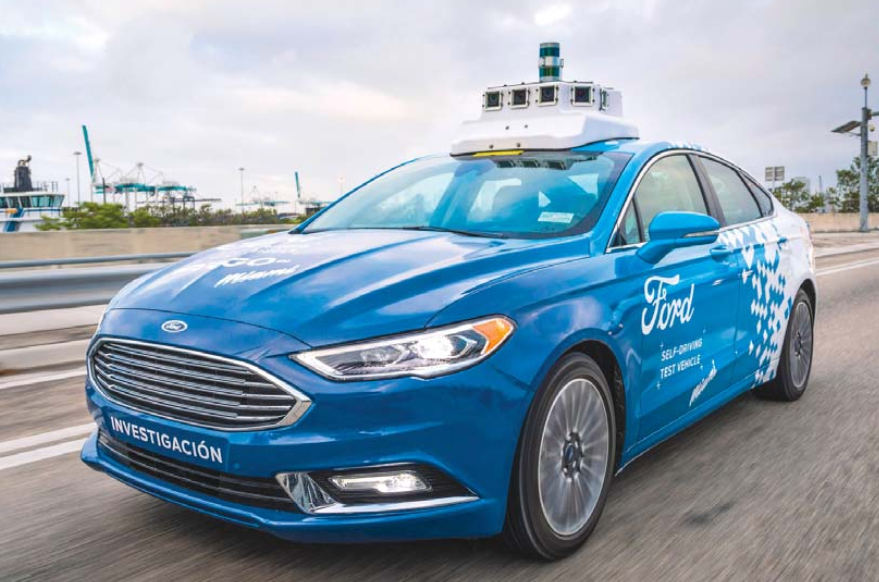
\includegraphics[width=467px, keepaspectratio]{imports/autonomous_vehicle.png}
        
        \caption{an example of an autonomous vehicle, the Ford Argo}  \cite{mccormick_self-driving_2019}
    \end{figure}
\end{center}

\subsection{Sensors for the autonomous vehicle}

To be aware of its environment, an AV usually carries a big cumbersome sensor package, because, to be sure the vehicle will not miss any detail in its environment, sensors redundancy and diversity are fundamental.

\subsubsection{LiDAR}

Out of all of the sensors, LiDAR is the most important and expensive, it costs tens of thousands of dollars. It is composed of an array of semiconductor lasers and optical detectors mounted on a rotating platform in an enclosure. By emitting pulses of near-IR light and measuring the return time of reflections, the system calculates a point cloud of objects surrounding the vehicle.”\cite{mccormick_self-driving_2019} The image created is updated 10 times per second and locates objects in a range of 50-100m with a 2 cm precision.
\smallskip

Nowadays, most companies (except Tesla) who are developing self-driving cars use LiDARs, despite of their high cost, their precision is crucial for the vehicle to picture and reconstruct its environment.
\smallskip

“As the single most expensive [AV] component, LiDAR has been the focus of intense R\&D by industry.”\cite{mccormick_self-driving_2019} Today, they are interested in replacing its rotative architecture that is cause of failure. Different approaches are being taken like using electromechanical mirrors for example, they intend to “steer laser beams without bulk mechanical motion”\cite{mccormick_self-driving_2019} and might allow to focus beams on detected objects to acquire more information about them.
\smallskip

Another preoccupation about LiDARs is eye safety, wavelengths used by LiDARs (900 nm) are quite dangerous for retina so, for now, power is limited. LiDARs with a higher, safer, wavelength exist but they require very expensive rare metals.

\subsubsection{Radar}

However, LiDARs can be easily limited by bad weather conditions and are relatively short-ranged. Consequently, AVs also use radars ; radars can determine objects speed towards the car (thanks to Dopler shift) allowing the AV to detect pedestrians and other vehicles. Furthermore, radars are cheaper (they cost hundreds of dollars) than LiDAR and still work in poor weather conditions.

\smallskip
AVs combine LiDAR and radar data for two tasks. It determines position and orientation in space with more precision than the GPS by locating landmarks on a base map. It also identifies and tracks moving objects ; their position and speed are then determined using statistical algorithms. The main inconvenient of the first task is the high dependence to already existing highly detailed maps.

\subsubsection{Camera}

The last sensor used by AVs is camera. Cameras with different focuses are used (near, far). Images are then analysed by neural networks to detect and classify objects including spotlights, lines, streets signs, etc. These data are used to validate or cancel trajectories calculated from the LiDAR and radar data.

\subsubsection{Sonar}

Until recently, ultrasonic sensors (sonars) were limited to parking assist because of their limited range, but, long range sonars exist nowadays. As a result, researchers developed an AV using a long-range ultrasonic sensors system\cite{budisusila_review_2019} capable of adapting to the speed of the vehicle, and braking if objects are detected on its trajectory albeit considering the distance between the vehicle and other vehicles behind the it. Ultrasonic sensors also have the advantage to be cheap, easy to implement in most vehicles, and calculations to get range information of the detected object are simple.

\subsection{Algorithms and control systems}

AVs carry sensors in order to get information about their environment, but these raw data must be analysed and treated to ensure the vehicle reacts accordingly. They need especially a path planning algorithms to find the best path to their destination, and to take into account detected objects like pedestrians that might be on it.

\subsubsection{Path planning}

Path planning uses all the data retrieved by the previously presented sensors, it includes two levels: a strategic level (the higher one) that decides, for example, if the car should overtake another car or wait, and a tactical level (the lower one) that determines, for example, the optimal steering angle or speed needed to accomplish an optimal maneuver.
\smallskip

Sensors work at a higher rate than path planning. Path planning is done on board the vehicle because the vehicle needs the best reaction time.
\smallskip

GPU are used to maximize the processing speed because most calculations are similar and can be parallelized. They are also used to train neural networks with data collected by vehicles.

\subsubsection{Pedestrian detection}

A challenge is to detect the pedestrians, for example, crossing or walking along the road. Indeed, it is a moving target and it can behave unexpectedly, becoming a danger. A way to predict the move of a pedestrian is to only use detection i.e consider it as an object in front of the vehicle,  and then react. But another way has been researched \cite{sarcinelli_handling_2019}, the path tracking of pedestrian. The latter is better in decision making and provides a more efficient and safer driving experience.

\begin{center}
    \begin{figure}[ht!]
        \centering
        
        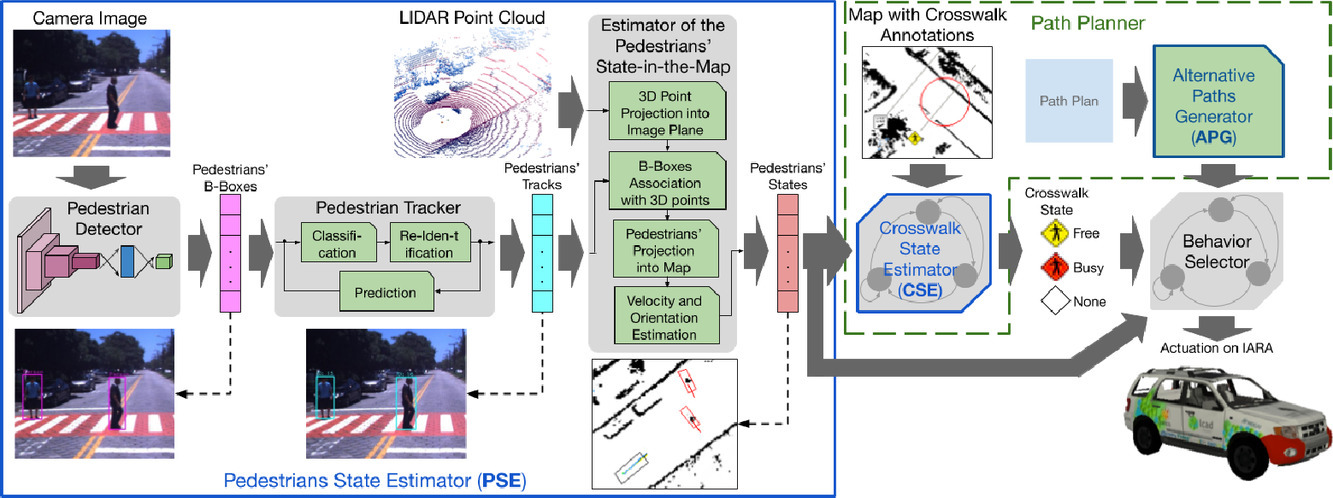
\includegraphics[width=467px, keepaspectratio]{imports/pedestrian1.jpg}
        
        \caption{Overview of the autonomous pedestrian detection architecture}  \cite{sarcinelli_handling_2019}
    \end{figure}
\end{center}

This technology allows to use temporal information for keeping track of the state (position, velocity, and orientation) of pedestrians, which allows the prediction of the near-future pedestrians' states (~3–5 s ahead).
\smallskip
The technology is divided in two main parts: the Perception System and the Decision-Making system. The first one is responsible for tasks of localizing the self-driving car, mapping of obstacles,tracking of moving obstacles, and recognition of traffic signalization. The second one is responsible for correctly driving the car according to the information provided by the perception system i.e control, path planning, behavior selection. 

\smallskip
In order to diminish the use of the Decision-Making part, many useful tasks to pedestrian detection are already performed at detection. The pedestrian boxes are calculated using a Convolutional Neural Network (CNN) in order to reduce the computational overhead, that is useful, considering that the detection of pedestrian is not the only computing that an autonomous car has to perform. For instance, YOLOv3 CNN \cite{redmon_yolov3:_2018} is one of the state-of-the-art systems for real-time object detection that is based on a bounding box (B-Box) regression, and include the Pedestrians’ Tracks which mainly classifies bounding-boxes of people present in scene as new or previously tracked person as seen in the figure 2.
\begin{center}
    \begin{figure}[ht!]
        \centering
        
        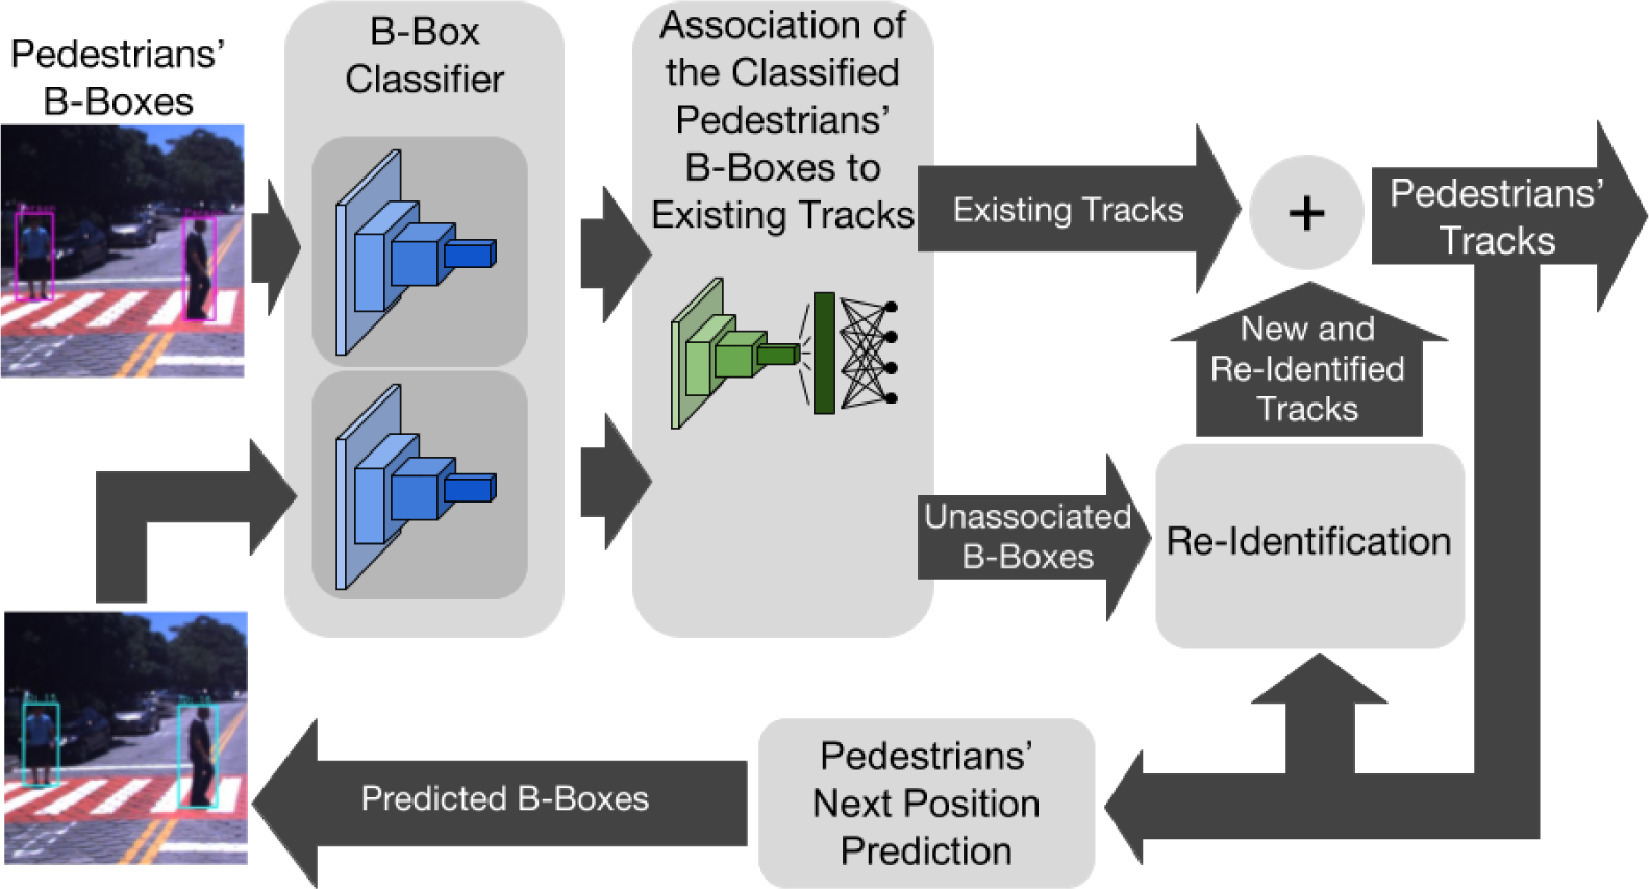
\includegraphics[width=467px, keepaspectratio]{imports/pedestrian2.jpg}
              \caption{Overview of the tracking system}
              \cite{sarcinelli_handling_2019}
    \end{figure}
\end{center}
First of all, the pedestrian boxes retrieves the camera picture from CCN, then we use LiDAR to get their position information in 3D, velocity and the accuracy of camera’s information (by providing others physics information) \cite{guidolini_handling_2018}. Pedestrians’ State-in-the-Map Estimator is the one who centralise all the LiDAR. It projects those 3D points collected by LiDAR into images, then calculate their real position by referencing the coordinate of the pedestrian boxes placed and the distance of the vehicle estimated , and finally provide a vector of triplets (position, orientation,velocity) to the decision making system to act accordingly.  
\smallskip

Finally, in the decision making part, the Crosswalk State Estimator (CSE) predicates the near future behaviour i.e whether the crosswalk is busy (has one or more pedestrians demanding right of passage) or free.
To perform that, the system is based on the car's velocity, the distance between the car and the crosswalk, and the presence of pedestrians around the crosswalk area and their walking speed/direction.
A state machine is used to predicate the pedestrians' intentions. To sum up,  intention exists if, and only if, the pedestrian is moving in the approximate direction (+/-30 degrees) of the center of the crosswalk area or is inside a crosswalk area and in the car’s path or  if velocity is equal or greater than 0.3 m/s and the pedestrian is not moving in the approximate direction (+/-30 degrees) of the road, meaning that he will perhaps cross the road soon. The angle range in both presented scenarios were empirically defined considering a normal human behaviour on these situations \cite{sarcinelli_handling_2019}.

There are a lot of methods to build an AV, on both hardware level and software level. Concerning the hardware, microprocessors/controllers units having GPIO ports (like arduino or raspberry pi) are used in recent studies. About the software, many algorithms are used like PID, fuzzy logic inference, and genetic algorithms, but the usage of neural network algorithms is quite rare.

\subsubsection{ADAS (Advanced Driver Assistant System)}

The ADAS is used in semi-automatic cars, unlike the systems found in AVs, its goal is not to replace the driver, but to turn it into an observer who monitors the movement of the car.

\subsubsection{Ultrasonic sensor system}

In 2004, a team designed "an ultrasonic sensor system to prevent accidents on the sides of the vehicle."\cite{budisusila_review_2019} The system was designed to be used in town at a speed of around 40 km/h, and sensors had a 6 meters range.

\subsubsection{ACC (Adaptive Cruise Control)}

The ACC system is used for longitudinal control of the vehicle (acceleration and deceleration), it takes three inputs:
\begin{itemize}
    \item Vehicle speed
    \item Driver setting time
    \item Distance measured by sensors (radars, sonars)
\end{itemize}
For an AV to follow another vehicle and stay at a reasonable distance, a new reference speed is calculated by the controller in a loop.
\newpage

\section{Opportunities and risks of autonomous vehicle}


\subsection{Autonomous Vehicle: Opportunity for urban mobility}
"Urban mobility is a dynamic system that has had a (slow) natural evolution" \cite{medina-tapia_exploring_2018}. With the development of technology, manuals vehicles will be replaced by AVs and vehicles will have the capable communicate and cooperate with each other. The society will expect significant innovations in mobility services. Moreover, the way people move around the urban environment is primed for profound changes , and cities will progressively become Smart Cities which will permit the vehicles to interact with the urban infrastructure.
The main goals of AV are to create a safer, more reliable, more efficient, more comfortable and more affordable way of travel. It is also expected to reduce traffic congestion, gas emission, fuel consumption, etc. When the autonomous system is activated, "the driver is replaced by a computer system to improve specific dimensions of driving such as safety, traffic fluidity, ecology, and economy".\cite{chehri_autonomous_2019} \smallskip

\begin{center}
    \begin{figure}[ht!]
        \centering
        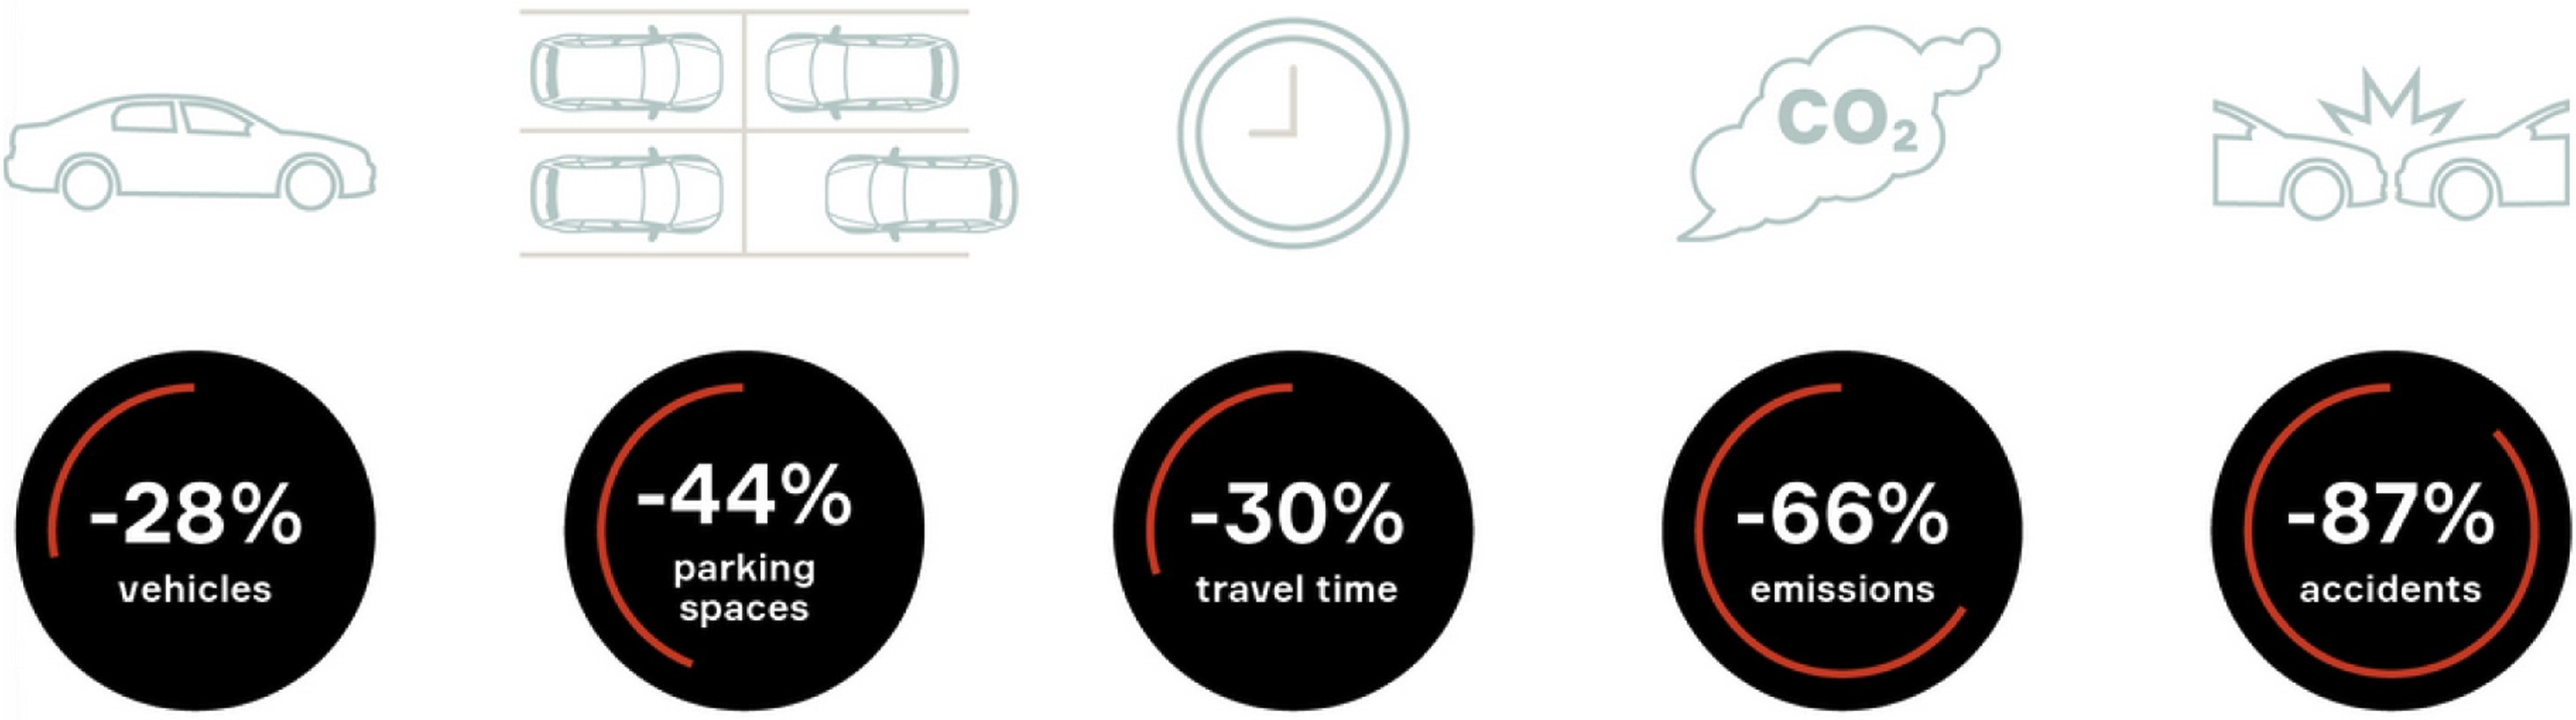
\includegraphics[width=400px, keepaspectratio]{imports/benefi_of_AVs..jpg}
        \caption{The benefit of autonomous vehicle in sustainable cities.}  \cite{chehri_autonomous_2019}
    \end{figure}
\end{center}

First of all, the automatization of the driving process (AVs) could reduce the generalized travel cost and the traffic congestion. Simulation studies show that AVs are capable of reducing collision on the road by eliminating or minimizing human errors and improving flow management, it could also make the real time-navigation more efficient. As a consequence, the AVs will allow increasing the urban road capacity due to platoon formations in urban roads and will reduce the amount of vehicle by 30\% in crowded city. Furthermore, they will increase the efficiency of infrastructure through better vehicle control. \smallskip

Secondly, the operation of transit and mobility services can be improved. The shared routes for theses services will be more accessible, reliable, and flexible. The AVs can make the mobility services more affordable and the transit operation by public services less subsidized. So that the transport services are increasingly capable of improving safety, reliability, security, and productivity. It could also benefit the citizen by offering an alternative mode of transportation and perhaps more efficient.\smallskip

Thirdly, the autonomous technologies can reduce greenhouse emissions by two third, thus reducing the pollution. The AVs make vehicles and infrastructure more environmentally friendly. It also encourages the transition from personal ownership to carpooling services. The ownership of the vehicle will be less necessary or unnecessary for users. Therefore, the number of vehicles will be reduced. The Avs could eliminate the waves of traffic created by stop-and-go behavior (where humans, rather than road accidents, create changes in speeds). This in turn will not only save people time, but decrease the time their cars are on the roads and therefore reduce emissions. \smallskip

Fourthly,  the AVs improve road safety. Beside of reducing traffic accidents by eliminating or minimizing human errors, it can make the journey less stressful and more comfortable. The United States Department of Transportation (USDOT) predicts that autonomous technologies has the potential to reduce traffic accidents by 87\%. \smallskip

Furthermore, the AVs have some other contribution to user, sustainable and cities and society. They benefit minors, the elderly, disabled, tired, drunk, or inattentive people by providing a greater freedom of mobility. Many seniors and people with disabilities cannot currently drive, even with vehicle modifications that help others drive safely. AVs could provide many more users access to the open road and to independence. It improves care and services dedicated to reduced mobility people. In addition, AVs can increase the life span of the vehicle by reducing the travel time . As a result, the maintenance cost can be reduced greatly.



\subsection{Challenges autonomous vehicles need to be overcome }

\subsubsection{Difficulty of understanding human gesture}

In the paper \cite{brooks_robotic_2017} the author discussed the difficulty for an autonomous car to understand human gesture. Figuring out of the way people pause and move is one of the problems yet to be solved even though some pedestrian detection mechanism have been mentioned in the previous part. An AV cannot tell what any human driver could decide instantaneously. For instance, the human driver can tell that people chatting on the street side have no intention to cross the road. On the other hand, if one suddenly turns away from the other in the direction of the street, it means that he or she is about to cross.
In the above situation, AVs lack the ability to assess the road safeness to move on. Should the AV decide, for safety reasons, to let the person start crossing the road by slowing down the vehicle or eventually coming to a halt in order to avoid hitting the person. Undoubtedly, this will slow down the traffic. If the person’s intention is guessed wrongly, the course of action will annoy the human driver that is stuck behind the autonomous cars. AVs would then create inconvenience.


\subsubsection{Anti-social act}

The flip side of AVs is giving the owners the opportunity to be anti-social. People will be tempted to take advantage of the road with their AVs without consideration for others. For instance, people will hop out of their cars in front of the shop to get something while leaving the car at an illegal parking spot, knowing well that AVs will take care of themselves and get out of the way if someone’s way is blocked. As a result, the traffic will be slowed down by this selfish act of the car owner and increase greenhouse gases emissions. Unattended cars will be everywhere.

\subsection{Implementation of security measure on an autonomous vehicle}

\subsubsection{Multi-layer IDS for autonomous vehicle}

A paper \cite{straub_cybersecurity_2017} described several component systems which comprised of an AV intrusion detection system (IDS) to detect suspicious activities, ranging from conventional local attacks to complicated manipulation attacks which are designed to manipulate the actions taken by the car. The multi-layer IDS proposed consists of four layers:
\begin{itemize}
  \item Vehicle-level intrusion detection. This IDS performs analysis on information without accessing to the larger network so it could be used to evaluate the trustworthiness of the network resources. However, this level is limited to the attacks that it can detect and the symptoms that it consider malicious as it does not try to compare data. Analysis performed are based on the data collected by the car to identify trends and patterns. The concept of mutually verifiable information implies that the user’s car can verify the information sent by the other car using their own sensor.

  \item Vehicle area network intrusion detection. This IDS scans the data transmitted between vehicles in real time with Vehicular Ad-Hoc Network(VANET) to look for anomalies and signs of malicious activity.
  
  \item Wide area vehicle coordination and traffic management. The third level securing information beyond the local VANET, using the roadside units (RSUs) for collection and transmission of data.
  
  \item Multiple areas or multiple layers of self-driving vehicle manipulation detection. 
\end{itemize}

\subsubsection {Reputation rating }
The reputation rating defines the trustworthiness of a car, the higher the reputation, the more likely the data emitted by the car will be taken into consideration of the analysis and calculation. If the rating drops below a certain level, it will be considered suspicious. Falling below limit, it will be categorized as malicious. The node with the highest rating serves as the gateway nodes to other proximate VANETs.

\subsubsection{Implementation difficulties}
This proposed IDS relies greatly upon the presence of RSUs but the feasibility of implementing RSUs cannot be adequately predicted at this time. Besides, the effectiveness of IDS will depend on the level of collaboration and coordination between vehicle manufacturers and their level of sharing of knowledge. 

Moreover, the authority who controls the cybersecurity responsibility (beyond the car level) will undoubtedly impact the priority of the cybersecurity system, the way it operates, and the configuration.
\newpage

\section{Communication View}

The autonomous cars need to gather information on their environment. This can only be done through a multiple exchanges between the vehicles but also with a centralized station. Therefore, the vehicles must be able to communicate  with other systems. In this part, we will study different protocols used for communication.

\subsection{Automotive software in connected vehicles}

In 2020, we estimate that 75\% of the cars will have the capacity to connect to the Internet, with a connectivity with connected object as smartphones.The article \cite{connectivity_car}, written by Hrvoje Vdovic from the Faculty of Electrical Engineering and Computing, University of Zagreb, Zagreb, Croatia, makes a review of the different information and communication technology (ICT) for connected and autonomous electric vehicle (CAEV).

The paper describes the softwarized architecture with a high level point of view. The system is composed by Electronic Control Units (ECUs) which is responsible for vehicle’s functions. The networking of ECUs is made with automotive bus system divided in 4 communication group: event-triggered bus systems, time-triggered bus systems, subnetworks and multimedia bus systems. The Control Area Network (CAN) is an event-triggered bus mainly used for real-time soft.

With connected vehicles, we can see 4 mainly types of communication:

\begin{itemize}
    \item Vehicle to Vehicle (V2V)
    \item Vehicle to road infrastructure
    \item Vehicle to Internet
    \item Vehicle to smart device
\end{itemize}

The internet communication is achieved either by a Telematics Control Unit, a module with a card SIM permanently installed, or by a modem which allows the use of a personal SIM card or either by a user’s smart device. 4G mobile communication allows communications with Internet and the communication with a smart device by a Bluetooth or Wi-Fi connection.

In the future, the automotive software development tends to aim four different goals: energy and cost efficiency, zero accidents, seamless connectivity and personalization. The paper identifies the main technological trends in automotive software:

\begin{itemize}
    \item Computer architecture centralization (decrease the number of ECUs and undesired interaction)
    \item Standardized communication, Ethernet may replace the current communication buses
    \item Connectivity and cooperation, challenges are the smart device communication and V2V communication
    \item Autonomous functions
\end{itemize}

\subsection{V2I}

Communication with infrastructures offers many new options to manage traffic. We will develop a solution based on V2I communications among others \cite{v2i_management}.

They used a local control station to collect information from the infrastructures or the vehicles to determine a driving state based on vehicles' information and road layout. The station controls the following:
\begin{itemize}
    \item The classification of vehicle within the driving area
    \item Identify stopped vehicle
    \item Inform every vehicle the modification of current speed or if overtaking is possible in straight road
    \item Provide information about road layout in bend stretches
    \item Identify traffic situation of risk
\end{itemize}

Researchers studied  V2I communication in order to manage the traffic flow. They defined two data packages for information exchange (the Reserved field can be used to exchange other information depending on the context): 

\begin{center}
    \begin{figure}[ht!]
        \centering
        
        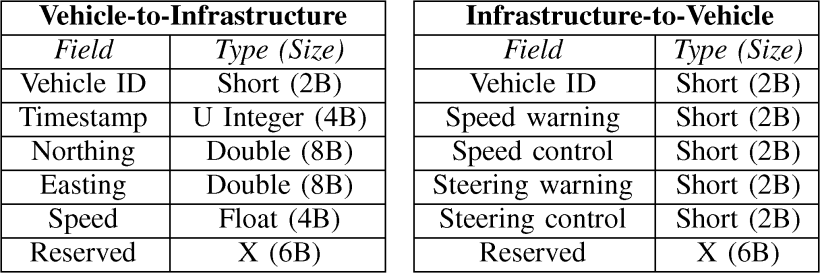
\includegraphics[width=400px, keepaspectratio]{imports/data_package_v2i_communication.png}
        
        \caption{Communications Data Packages}  
        \cite{v2i_management}
    \end{figure}
\end{center}

The communication is achieved by WAVE \cite{v2i_management} communication based on IEEE 8021.11p standard that proposes enhanced distributed channel access (EDCA). EDCA defines four different traffic classes with different priorities:  AC\_VO (Voice Access Category),AC\_VI (Video Access Category, generally unused),  AC\_BE (Best-Effort Access Category) and  AC\_BK (Background Access Category). AC\_VO can only be used by few vehicle and so is kept to special situation as emergency. The challenge is to maintain the delay and packet-loss under a certain limit.
\smallskip

A higher layer mechanism on top of the WAVE stack must be build for critical message dissemination. Unfortunately, the conditions of this applications involve that to maintain the quality of service and real-time application, the number of stations must be less than 40.

\smallskip

In order to handle every kind of situations that can occur, the control station gives the same importance to each car. The car use the collected information they need to make decision. These information are mainly the distance to the vehicle ahead and its velocity. The information is then compared to the references and adapted to their behavior properly. The driving state is also sent by the control station so that the car is aware of the current level of risk.

\smallskip

The driving state \cite{v2i_management} of the car is ranged between -1 and 1 which illustrates the compromise between safety and traffic flow: 0 represent the perfect compromise whereas -1 stands for safe but poor traffic flow and 1 represents the presence of risk of car accident. Therefore the cars try to keep their driving state a little under 0 to ensure the safety of the vehicle.

To check if the driving state was reflecting the real behavior of the car, the researchers tested several scenarios if the car exceeded the recommended velocity. As mentioned in the figure below, the results showed that the driving state was coherent with the situation: when the car exceeded the target velocity, the driving state got closer to 1 and it resulted in a collision.

\begin{center}
    \begin{figure}[ht!]
        \centering
        
        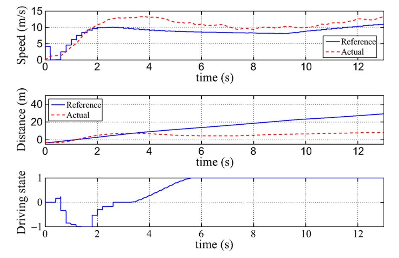
\includegraphics[width=400px, keepaspectratio]{imports/graph_driving_state.png}
        
        \caption{Coherence of the driving state with the situation}  
        \cite{v2i_management}
    \end{figure}
\end{center}




\subsection{oneM2M Standard}


OneM2M was created in 2009 by a group of seven organizations working in the field of standards and industry \cite{alaya_toward_2015}
The main purpose of the oneM2M standards is to unify the different “M2M isolated services” into one norm used by everyone.
\smallskip

A oneM2M system is modeled by four types of nodes: “application dedicated node (ADN), application service node (ASN), middle node (MN), and infrastructure node (IN).” \cite{alaya_toward_2015} An application node is high level whereas an infrastructure node is low level.

oneM2M also aims to solve the problem of interoperability definitively so that those connected object should be able to communicate with another one even if it is a heterogeneous device.
\smallskip

However, oneM2M standard initially does not include semantic data. In other words, data used by oneM2M are not standardized using an ontological model. Ontology is the way to structure data for example adding meta-data in order to specify their semantic. Therefore it was difficult for the applications to understand the meaning of the data exchanged. That was one of the reasons why OM2M was created.


\subsection{OM2M Framework}

OM2M is a framework which aims to make the development of IoT applications easier. It was developed by three researchers of the LAAS-CNRS: Karima Khadir, Thierry Monteil and Samir Medjiah \cite{SicariSabrina2015SOSP}. As the name implies, it respects the oneM2M standard.
\smallskip

This framework proposes that a server should gather the information of each sensor and the data collected from the sensors by the IDE-OM2M.
The OM2M platform has several functionalities:  
\begin{itemize}
    \item Automatic discovery of connected devices
    \item Notification of subscribers to the arrival of new events
    \item Efficient routing 
\end{itemize}
It also uses the HTTP standard in order to exchange data through GET requests for instance.
\smallskip

OM2M has several benefits over other platforms: One of them is syntactic and semantic interoperability. It enables the applications to "understand" the meaning of the information they received from other devices. OM2M added two options to describe the semantic of a resource.
Secondly, this architecture is decentralized because one device can use several OM2M platforms which is not the case for other platforms.
\smallskip

It also has a graphical environment based on Node-RED and it is very intuitive for the user. Nevertheless, several softwares and platforms already developed and used their own framework. The article also listed nine alternative frameworks. Therefore, we can always find a suitable framework which suits to our needs.
\smallskip

The article provides us an example of application: Luminosity control in a building \cite{SicariSabrina2015SOSP}. One OM2M entity is used to collect the information of luminosity in the room. A Semantic Actuactor selects the lamp in the database which consumes the least energy. The lamps are lit until the specified limit is reached.
The article explains in the conclusion that they want to cooperate with NCTU University in order to develop the OM2M framework.
\newpage

\sectionnn{Conclusion}

Designing an autonomous vehicle is challenging in many ways, requiring several advanced technologies to mimic what a driver does. Nevertheless, the increase of computational power and the boosting IA development make AV a trend in the domain of research. It makes us believe that this technology will soon reach a mature state of development and eventually become reliable enough to be commercialised someday. Such an outcome could revolutionize the transport in reducing costs, traffic congestion and above all the accidents rate.
\smallskip

As the world continues to move progressively toward a transportation system driven by AV, what AV could bring up to the society is significant. 
AV has potential to transfer urban mobility by offering the opportunity for an efficient, safe, accessible and affordable transportation. They promise not only an alternative system of mobility but also a new approach to the urban lifestyle. Even though these benefits are far from guaranteed.
\smallskip

The existing technologies today allows us to detect obstacles and road condition by reconstructing the environment from pictures (by using cameras) or from points (by using LiDAR). However, the body gesture of the pedestrian is not taken in consideration of the calculation. Pedestrians are "seen" only as an obstacle under the eyes of the sensors. 

\smallskip

%platform connecte(Remy) - connectivity(denis)
The communication between connected cars is a not a piece of cake. The communication of AV is based on different layer : communication vehicle to vehicle, communication vehicle to road infrastructure, communication vehicle to smart device or communication vehicle to Internet. Communication of vehicle to infrastructure allows control stations to manage driving areas and improves GPS application or even to detect violation such as red light violation.
\smallskip

We studied the OM2M framework in particular. It is based on the oneM2M standard and makes possible to precise the semantic of the information exchanged between devices. It offers a graphical interface to make it easier to use. Therefore, it is the framework we are going to use for our project.\smallskip

The INSA vehicle possesses LiDAR and camera that could be used to get information about the campus. For instance, it allows us to know the number of available parking slots and their positions, or the number of people queuing for the restaurant, or even analyses paths taken by students to get to class.
%===================================================================

\newpage
\pagestyle{fancy}
\lhead{}
\chead{}
\rhead{}
\lfoot{\projecttitle}
\cfoot{}
\rfoot{}

\bibliographystyle{IEEEtran}

\bibliography{imports/bibliography} 
\end{document}
%==[DO NOT CHANGE ANYTHING HERE]====================


